\documentclass[compress]{beamer}
\usepackage{ifthen,verbatim}

\newcommand{\isnote}{}
\xdefinecolor{lightyellow}{rgb}{1.,1.,0.25}
\xdefinecolor{darkblue}{rgb}{0.1,0.1,0.7}

%% Uncomment this to get annotations
%% \def\notes{\addtocounter{page}{-1}
%%            \renewcommand{\isnote}{*}
%% 	   \beamertemplateshadingbackground{lightyellow}{white}
%%            \begin{frame}
%%            \frametitle{Notes for the previous page (page \insertpagenumber)}
%%            \itemize}
%% \def\endnotes{\enditemize
%% 	      \end{frame}
%%               \beamertemplateshadingbackground{white}{white}
%%               \renewcommand{\isnote}{}}

%% Uncomment this to not get annotations
\def\notes{\comment}
\def\endnotes{\endcomment}

\setbeamertemplate{navigation symbols}{}
\setbeamertemplate{headline}{\mbox{ } \hfill
\begin{minipage}{5.5 cm}
\vspace{-0.75 cm} \small
\end{minipage} \hfill
\begin{minipage}{4.5 cm}
\vspace{-0.75 cm} \small
\begin{flushright}
\ifthenelse{\equal{\insertpagenumber}{1}}{}{Jim Pivarski \hspace{0.2 cm} \insertpagenumber\isnote/\pageref{numpages}}
\end{flushright}
\end{minipage}\mbox{\hspace{0.2 cm}}\includegraphics[height=1 cm]{../cmslogo} \hspace{0.1 cm} \includegraphics[height=1 cm]{../tamulogo} \hspace{0.01 cm} \vspace{-1.05 cm}}

\begin{document}

%% \begin{notes}
%% \item This is the annotated version of my talk.
%% \item If you want the version that I am presenting, download the one
%% labeled ``slides'' on Indico (or just ignore these yellow pages).
%% \item The annotated version is provided for extra detail and a written
%% record of comments that I intend to make orally.
%% \item Yellow notes refer to the content on the {\it previous} page.
%% \item All other slides are identical for the two versions.
%% \end{notes}

\small

\begin{frame}
\frametitle{News and Announcements}
\begin{itemize}\setlength{\itemsep}{0.35 cm}
\item Conversion of photogrammetry results to CSCAlignmentRcd: \mbox{\textcolor{darkblue}{ongoing}\hspace{-1 cm}}
\begin{itemize}
\item Karoly and Oleg are doing a proper accounting of the $z$ heights
  of pins to determine all $z$ positions and $\phi_x$ angles
\end{itemize}

\item Jim Bellinger's database comparison tool: \mbox{\textcolor{darkblue}{done, maybe minor fixes}\hspace{-1 cm}}
\begin{itemize}
\item compares alignment of chambers relative to a ring or disk
  between two prospective geometries: ideal for comparing track-based
  and hardware alignments in a local system
\item In CVS: \mbox{\tt \scriptsize Alignment/MuonAlignment/plugins/MuonGeometryArrange\hspace{-1 cm}}
\end{itemize}

\item Further developments in tracker alignment as seen from the muon
  system (slide 2)

\item Today: track-based validation and track-based diagnostics \mbox{(slides 3--4)\hspace{-1 cm}}

\end{itemize}
%% \hspace{-0.83 cm} \textcolor{darkblue}{\Large Outline2}
\end{frame}

%% \section*{First section}
%% \begin{frame}
%% \begin{center}
%% \Huge \textcolor{blue}{First section}
%% \end{center}
%% \end{frame}
\begin{frame}
\frametitle{Muon $Z$ residuals vs.\ $Z_{PCA}$}

\begin{itemize}

\item ``Outer'' plots require $R_{PCA} > 58$~cm, ``inner'' plots require $R_{PCA} < 58$~cm and APE = 1000~cm ($\approx \infty$) in TOB and TEC

\item Muon $Z$ residuals in mm: tracker displacements are smaller

\mbox{ } \hfill \scriptsize \begin{tabular}{c | c c c c c}
& minus TEC & plus TEC & TOB & TIB & TID \\\hline
bottom & $+9$ & $-4$ & $-1.3$ & $-0.4$ & not a good \\
top & $-0.6$ & $+3$ & $+2$ & $-0.9$ & track-fit? \\
\end{tabular} \hfill \mbox{ }
\end{itemize}

\vfill
\begin{columns}
\column{0.25\linewidth}
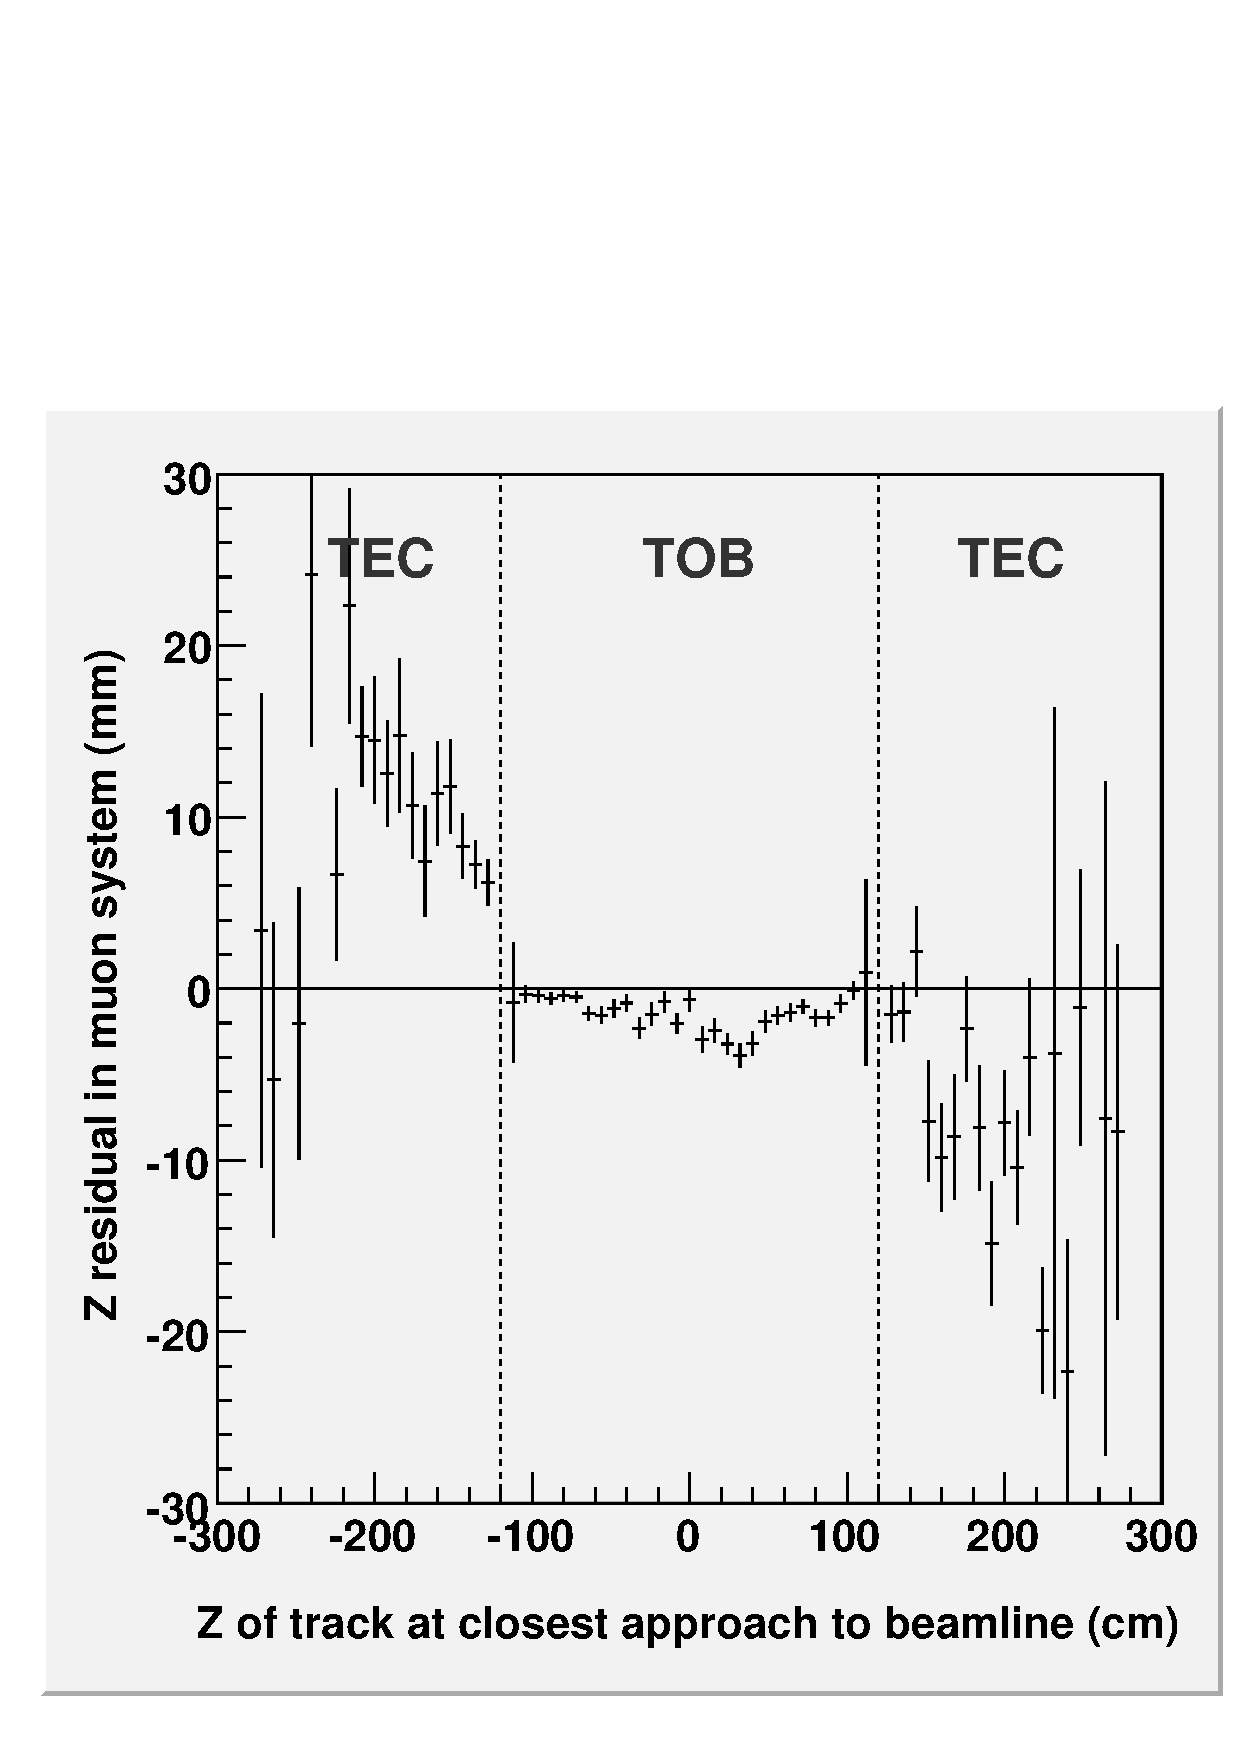
\includegraphics[width=\linewidth]{zresid_from_tracker_outerbottom.pdf}

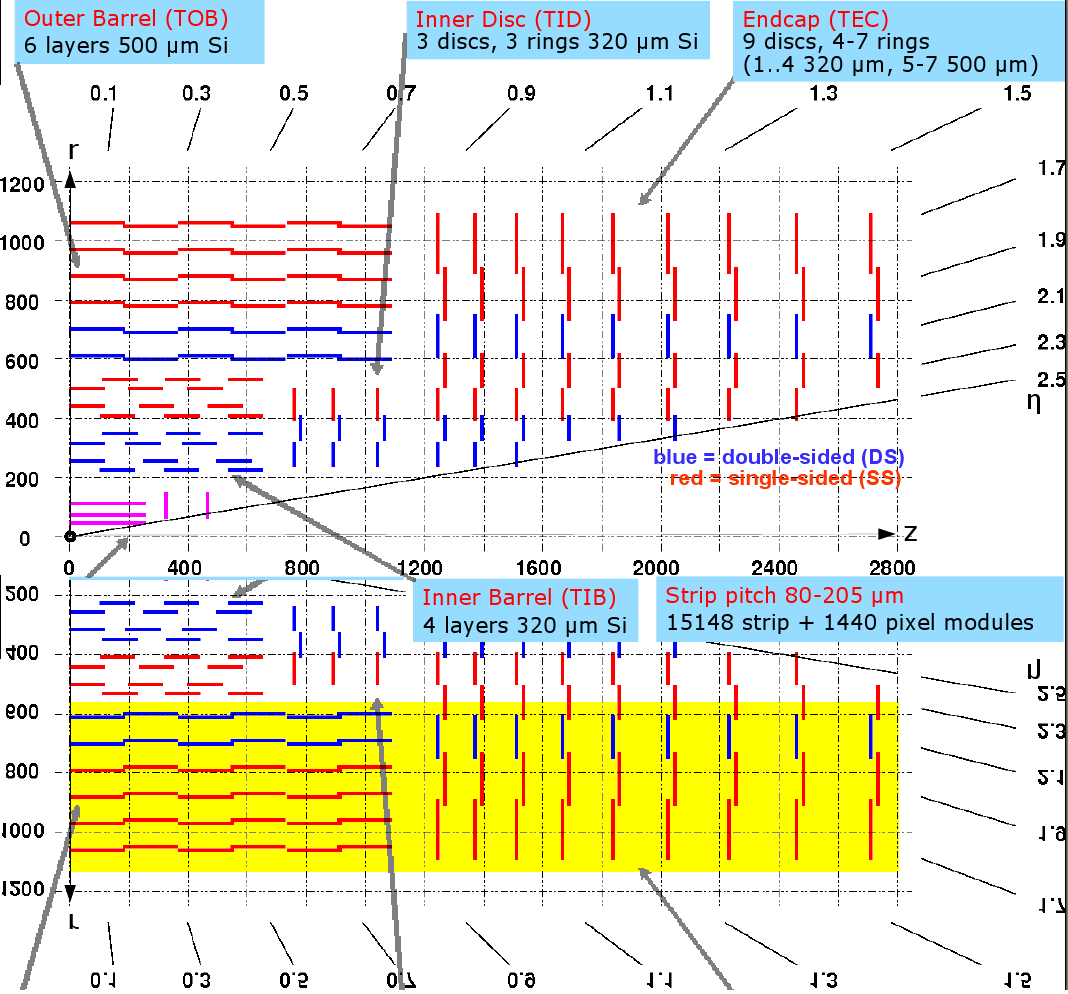
\includegraphics[width=\linewidth]{tracker_map_outerbottom.png}

\column{0.25\linewidth}
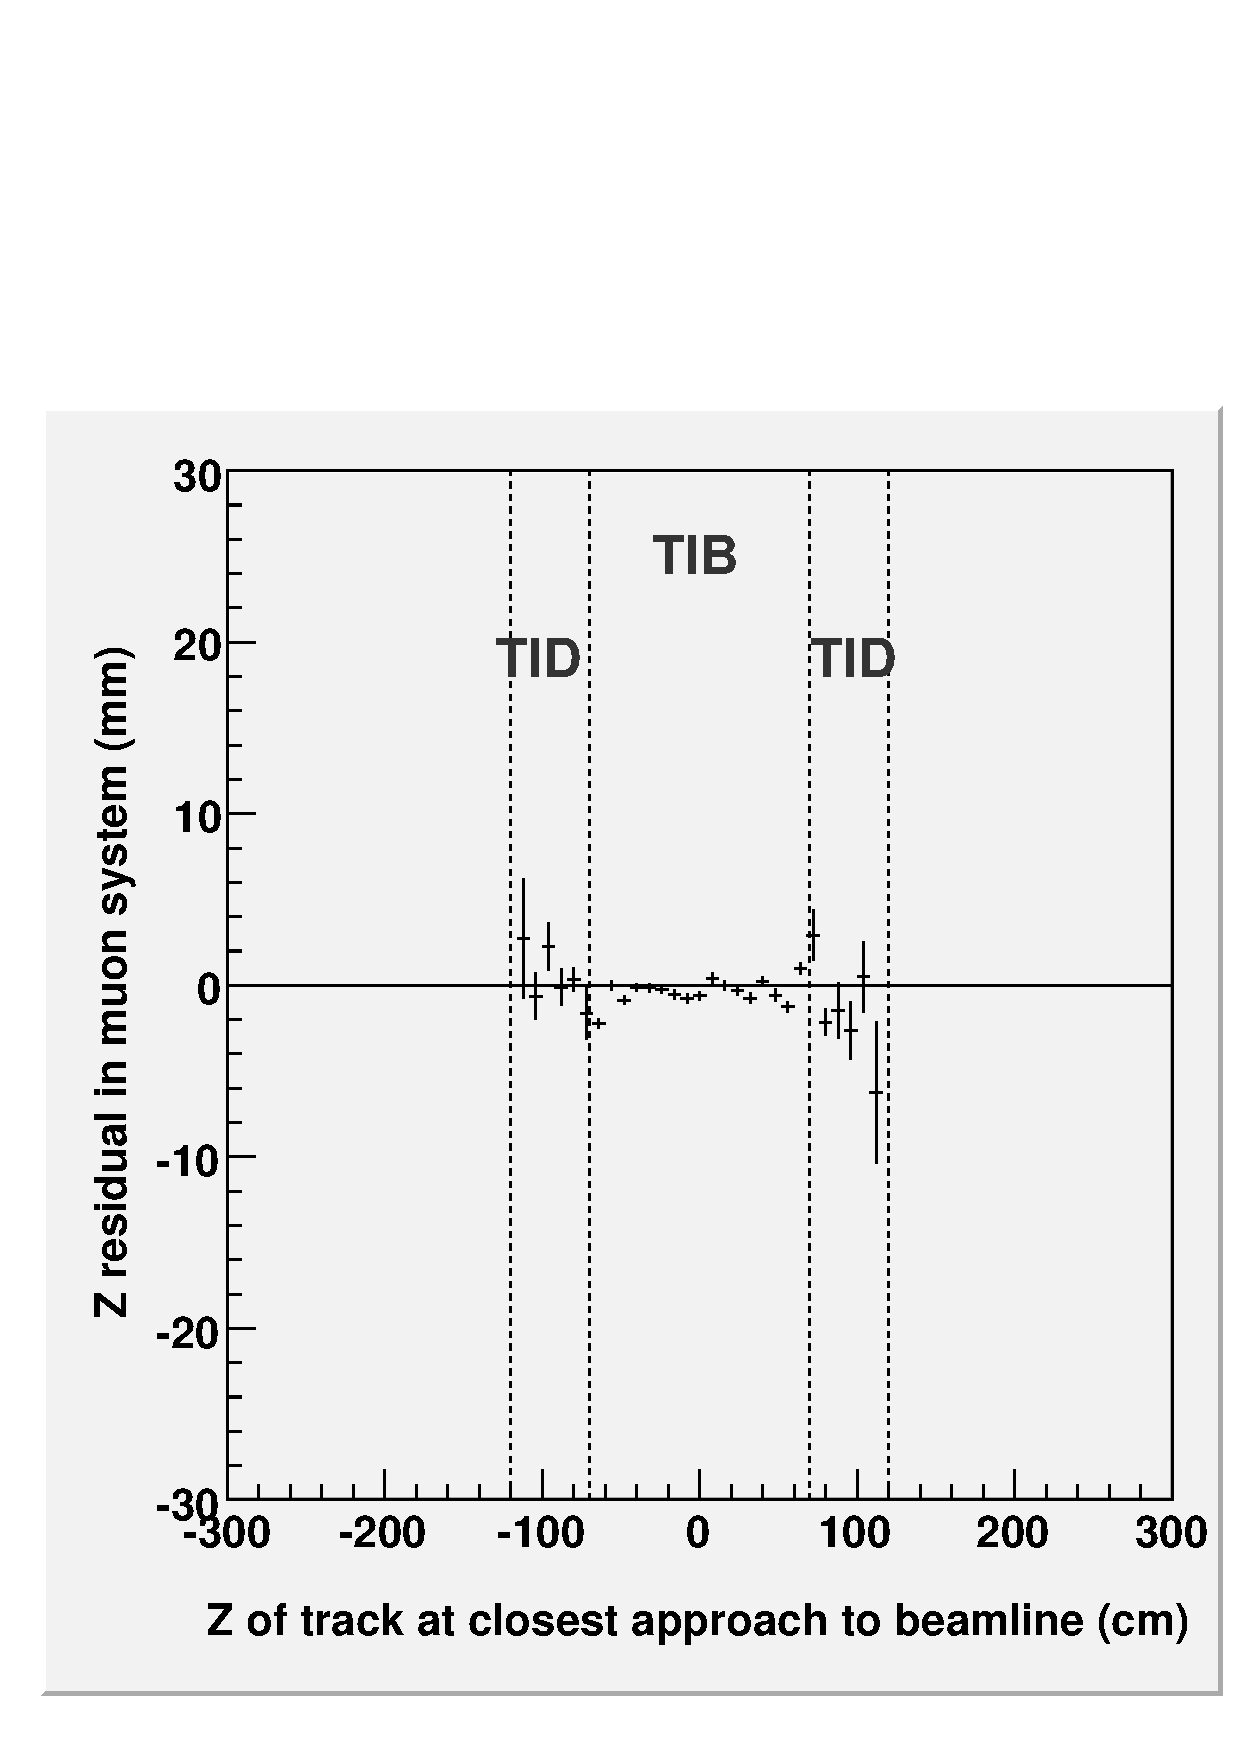
\includegraphics[width=\linewidth]{zresid_from_tracker_innerbottom.pdf}

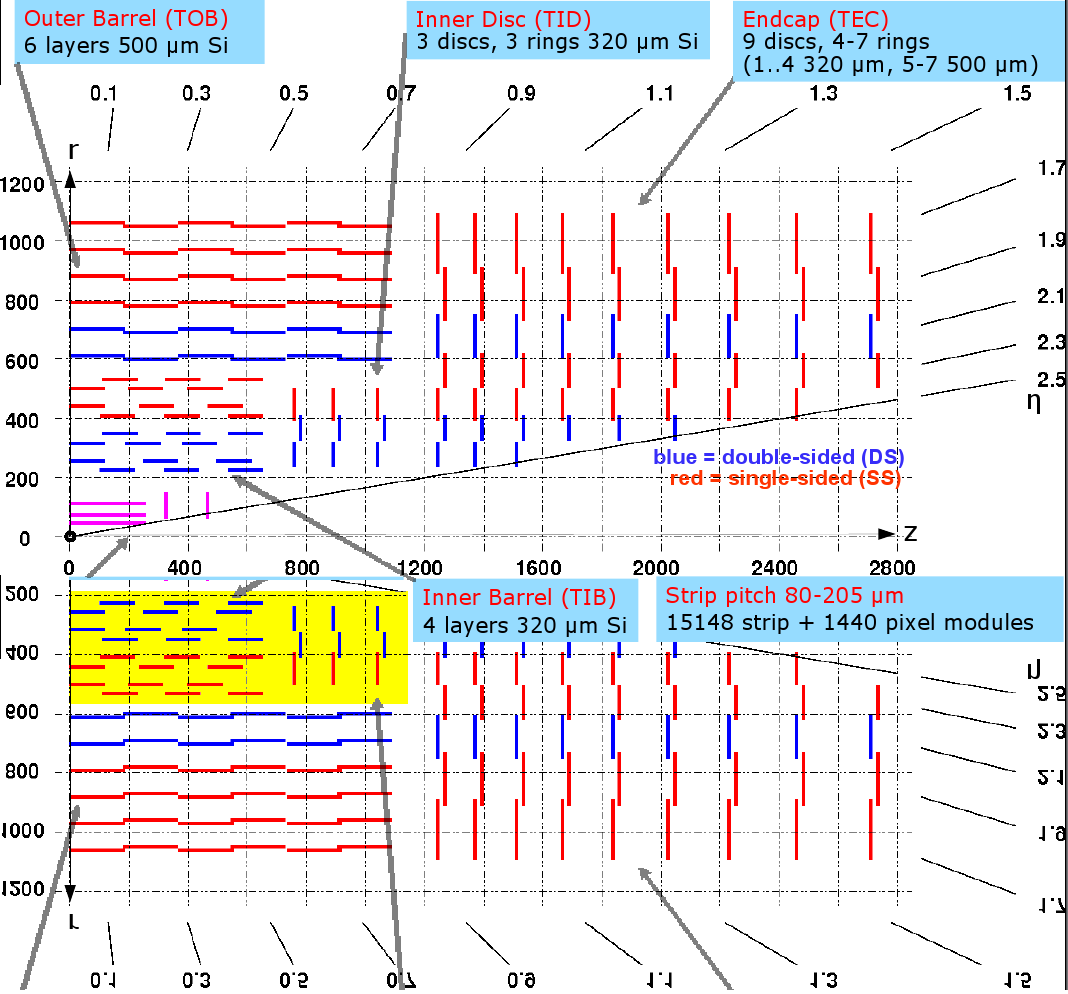
\includegraphics[width=\linewidth]{tracker_map_innerbottom.png}

\column{0.25\linewidth}
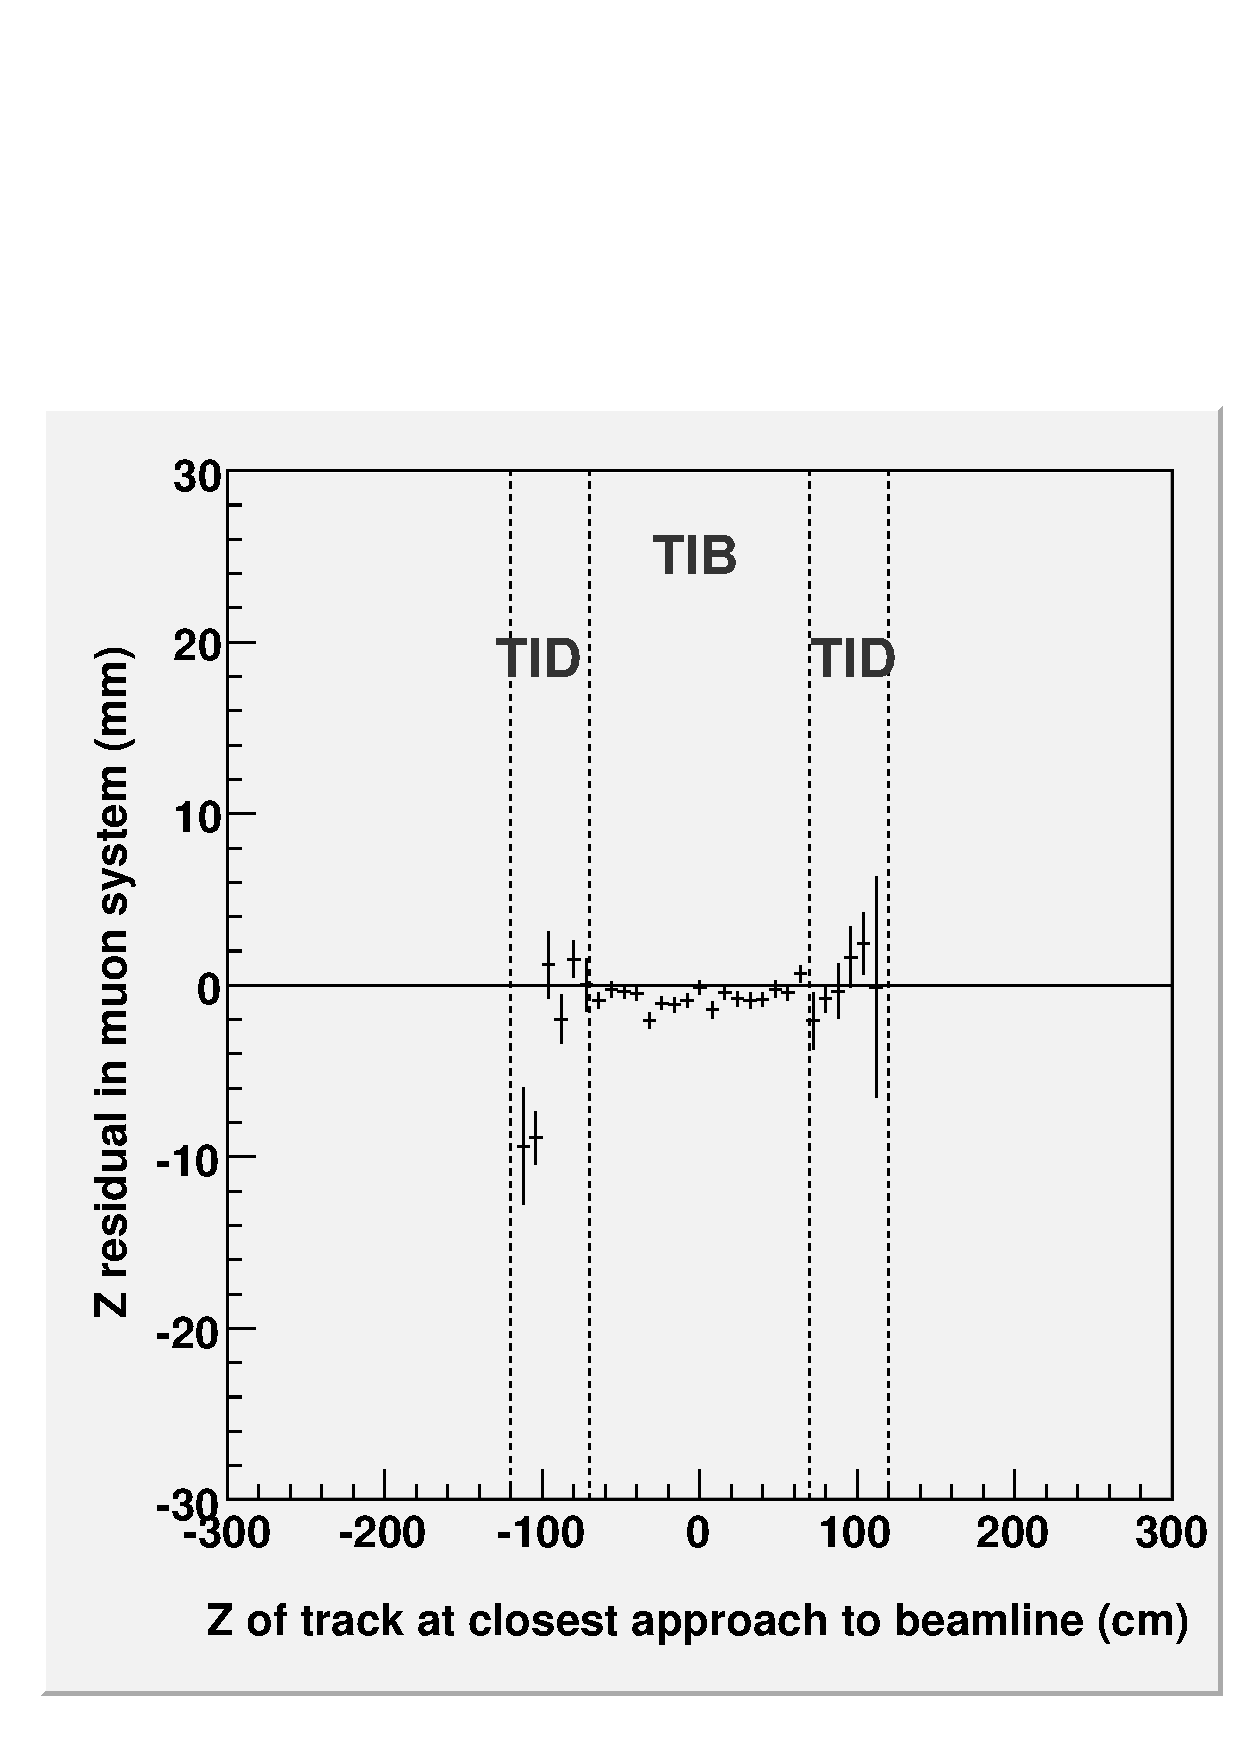
\includegraphics[width=\linewidth]{zresid_from_tracker_innertop.pdf}

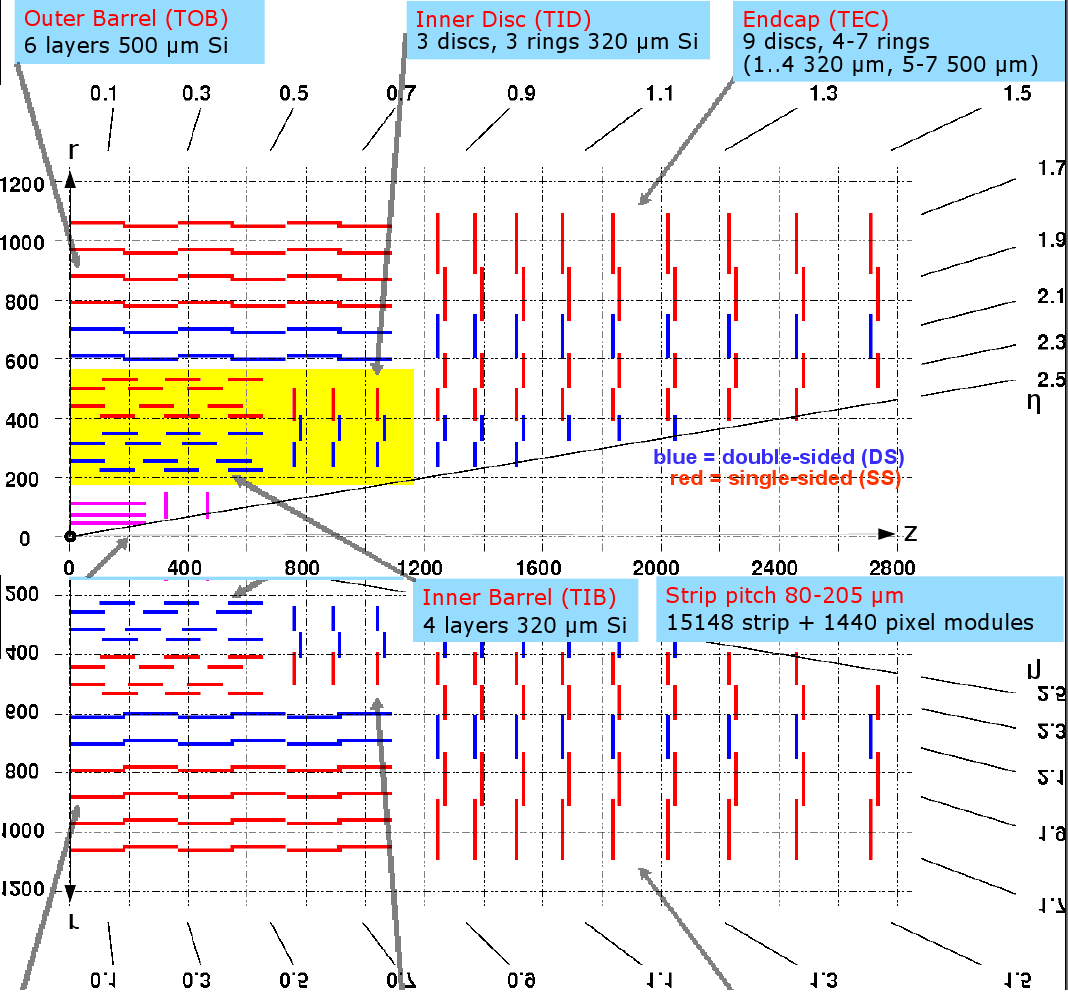
\includegraphics[width=\linewidth]{tracker_map_innertop.png}

\column{0.25\linewidth}
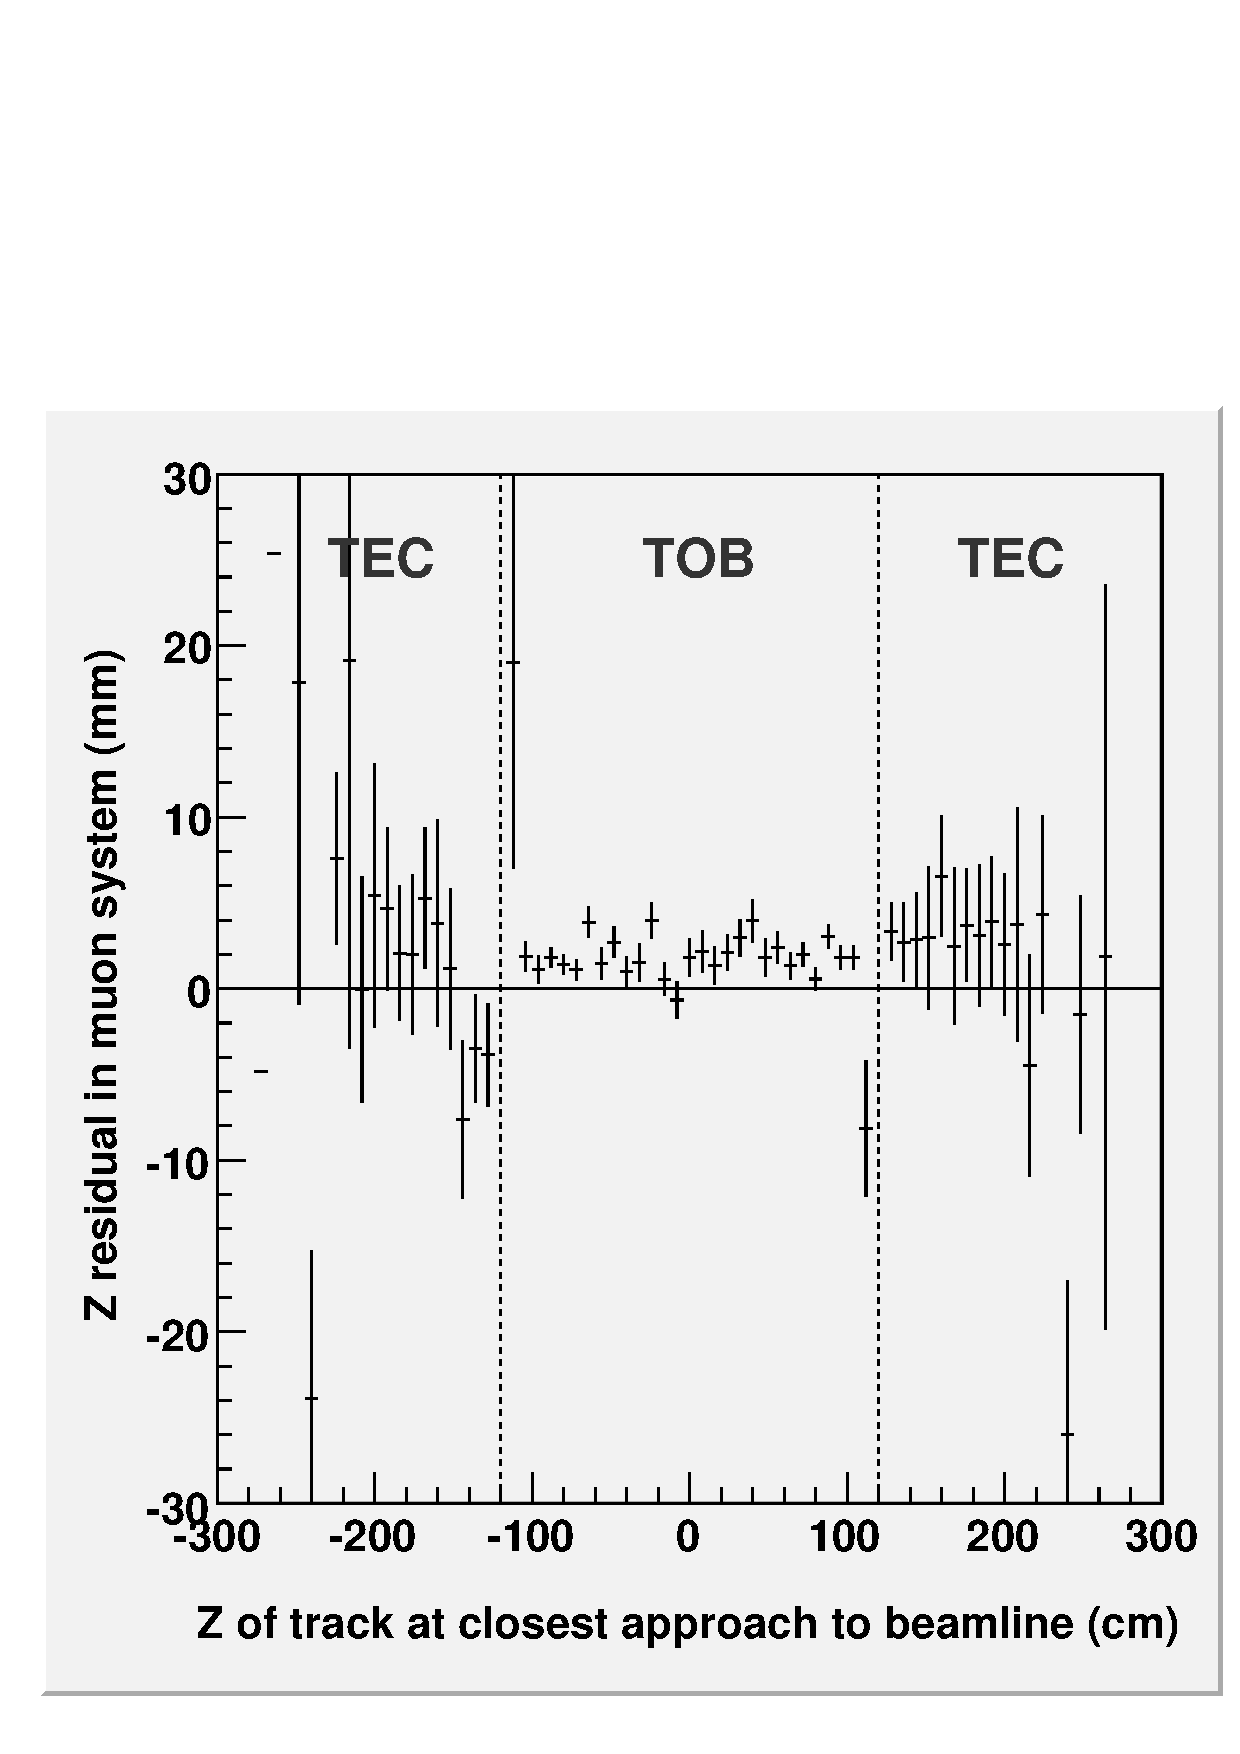
\includegraphics[width=\linewidth]{zresid_from_tracker_outertop.pdf}

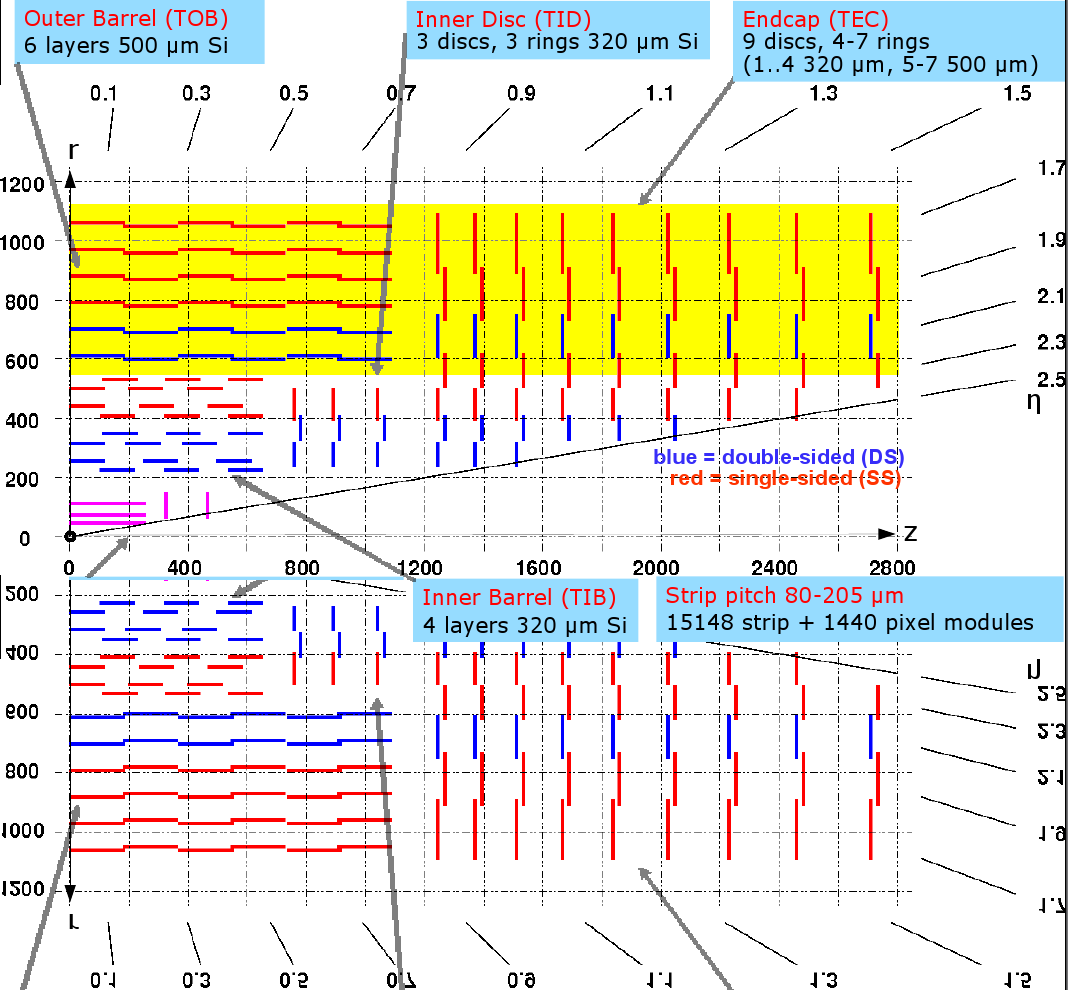
\includegraphics[width=\linewidth]{tracker_map_outertop.png}
\end{columns}
\end{frame}

\begin{frame}
\frametitle{Validation and diagnostics}
Before starting this discussion and Nick's talk\ldots

\begin{enumerate}\setlength{\itemsep}{0.1 cm}
\item I would distinguish
\begin{itemize}
\item \textcolor{darkblue}{validation:} check for surprises on a routine basis in DQM

$\longrightarrow$ a safety net for catching mistakes

\item \textcolor{darkblue}{diagnostics tool:} check parts of the alignment in different ways%, e.g.

\end{itemize}

\item While the residuals RMS or track $\chi^2$ is a good measure of misalignment in
  the tracker, it isn't in the muon system
\begin{itemize}
\item track error matrices $\gg$ misalignments due to \mbox{propagation in iron\hspace{-1 cm}}
\item makes residual $\sim$ intrinsic error ($\oplus$ internal \mbox{layer misalignments)\hspace{-0.5 cm}}
by construction, after the first hit in each chamber
\item segment residuals overcomes this issue, but then there are only
  four ``hits'' in the track-fit: they each have significant pull
\end{itemize}

\item Only good measure of misalignment in muon system that I know of:
  mean of residuals from hits excluded from fit
\begin{itemize}
\item distribution of means is much more sensitive than RMS of combined distribution, though we don't have \mbox{many alignables\ldots\hspace{-1 cm}}
\end{itemize}

\item Ideally, validation and diagnostics should refit AlCaReco

\end{enumerate}
\end{frame}

\begin{frame}
\frametitle{Examples of cross-checks}

(Didn't fit on the previous slide)

\vfill
\begin{columns}
\column{0.5\linewidth}
\scriptsize globalMuons vs.\ \mbox{standAloneMuons\hspace{-1 cm}}

\vspace{0.1 cm}
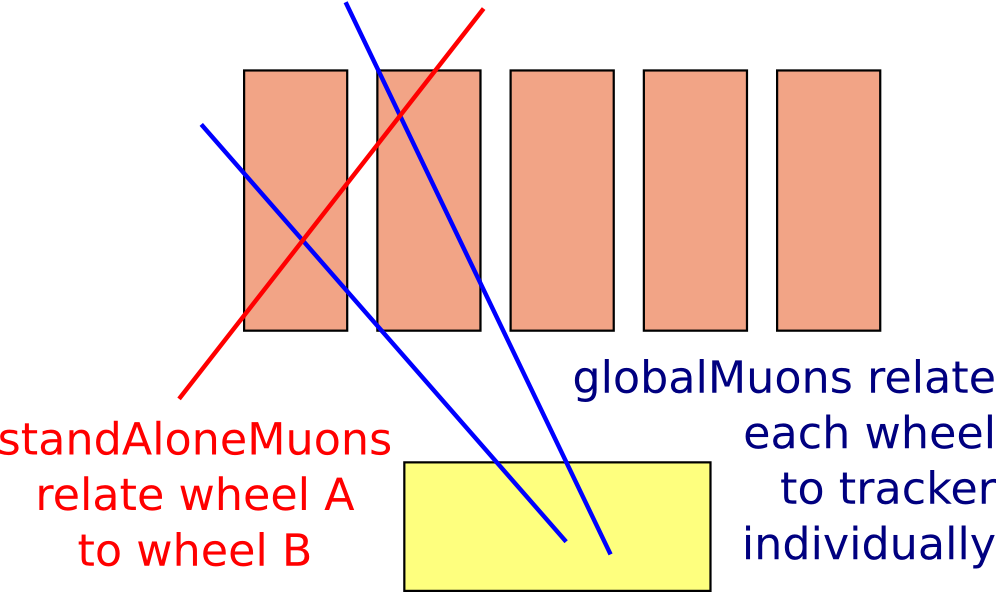
\includegraphics[height=3 cm]{globalMuon_standAloneMuon.png}

\column{0.5\linewidth}
\scriptsize CSC overlaps vs.\ \mbox{straight-through tracks\hspace{-1 cm}}

\vspace{0.1 cm}
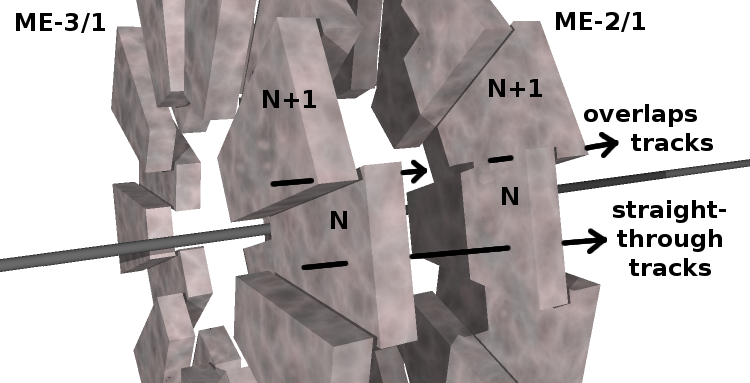
\includegraphics[height=3 cm]{overlaps_straight_through.png}
\end{columns}

\vfill
\begin{itemize}\setlength{\itemsep}{0.1 cm}
\item StandAloneMuon positions of wheels A and B must be equal to the difference of globalMuon positions
\item Helps us track down potential sources of bias in globalMuons measurement
\end{itemize}
\label{numpages}
\end{frame}
\end{document}
